\documentclass{article}
\usepackage[utf8]{inputenc}

\usepackage[T2A]{fontenc}
\usepackage[utf8]{inputenc}
\usepackage[russian]{babel}

\usepackage{tabularx}
\usepackage{amsmath}
\usepackage{pgfplots}
\usepackage{geometry}
\geometry{
    left=1cm,right=1cm,top=2cm,bottom=2cm
}
\newcommand*\diff{\mathop{}\!\mathrm{d}}

\newtheorem{definition}{Определение}
\newtheorem{theorem}{Теорема}

\DeclareMathOperator{\sign}{sign}

\usepackage{hyperref}
\hypersetup{
    colorlinks, citecolor=black, filecolor=black, linkcolor=black, urlcolor=black
}

\title{Дискретная математика}
\author{Лисид Лаконский}
\date{September 2023}

\begin{document}
\raggedright

\maketitle

\tableofcontents
\pagebreak

\section{Практическое занятие — 26.09.2023}

Импликацией, эквивалентностью, сложением по модулю два, коимпликацией, штрихом Шеффера и стрелкой Пирса называются функции, заданные, соответственно, следующими таблицами истинности:

$\begin{vmatrix}
    x & y & x \rightarrow y & x \sim y & x \bigoplus & x \leftarrow y & x | y & x \downarrow y \\
    0 & 0 & 1 & 1 & 0 & 0 & 1 & 1 \\
    0 & 1 & 1 & 0 & 1 & 0 & 1 & 0 \\
    1 & 0 & 0 & 0 & 1 & 1 & 1 & 0 \\
    1 & 1 & 1 & 1 & 0 & 0 & 0 & 0
\end{vmatrix}$

\subsection{Нормальные формы: ДНФ, КНФ, СДНФ, СКНФ, АНФ}

Можно составлять с помощью законов алгебры логики или таблицы истинности (или с помощью чего еще хочется). Допустим, имеем:

$\begin{vmatrix}
    x & y & z & f \\
    0 & 0 & 0 & 0 \\
    0 & 0 & 1 & 1 \\
    0 & 1 & 0 & 0 \\
    0 & 1 & 1 & 0 \\
    1 & 0 & 0 & 1 \\
    1 & 0 & 1 & 1 \\
    1 & 1 & 0 & 0 \\
    1 & 1 & 1 & 1
\end{vmatrix}$

\paragraph{СДНФ}

$f = \overline{x} \overline{y} z + x \overline{y} \overline{z} + x \overline{y} z + x y z$

\paragraph{ДНФ}

$f = x \overline{y} + x z + \overline{y} z$

\paragraph{СКНФ}

$f = (x + y + z)(x + \overline{y} + z)(x + \overline{y} + \overline{z})(\overline{x} + \overline{y} + z)$

\paragraph{КНФ} $f = (x + z)(x + \overline{y})(\overline{y} + z)$

\paragraph{Полином Жегалкина (АНФ)} Метод треугольника (часто называемый методом треугольника Паскаля) позволяет преобразовать таблицу истинности в полином Жегалкина путём построения вспомогательной треугольной таблицы в соответствии со следующими правилами:

\begin{enumerate}
    \item Строится полная таблица истинности, в которой строки идут в порядке возрастания двоичных кодов от 000…00 до 111…11.
    \item Строится вспомогательная треугольная таблица, в которой первый столбец совпадает со столбцом значений функции в таблице истинности.
    \item Ячейка в каждом последующем столбце получается путём суммирования по модулю 2 двух ячеек предыдущего столбца — стоящей в той же строке и строкой ниже.
    \item Столбцы вспомогательной таблицы нумеруются двоичными кодами в том же порядке, что и строки таблицы истинности.
    \item Каждому двоичному коду ставится в соответствие один из членов полинома Жегалкина в зависимости от позиций кода, в которых стоят единицы. Например, ячейке 111 соответствует член ABC, ячейке 101 — член AC, ячейке 010 — член B, ячейке 000 — член 1 и т. д.
    \item Если в верхней строке какого-либо столбца стоит единица, то соответствующий член присутствует в полиноме Жегалкина.
\end{enumerate}

АНФ для таблицы, представленной выше: $$f = z \oplus yz \oplus x \oplus xz \oplus xy$$

\subsection{Минимизация булевых функций: метод Куайна}

Минимизировать СДНФ булевой функции методом Квайна и по карте Карно. Привести к скобочной форме, построить логическую схему. Пусть функция трех переменных, задана таблицей истинности:

$$\begin{vmatrix}
    n & x & y & z & f \\
    0 & 0 & 0 & 0 & 1 \\
    1 & 0 & 0 & 1 & 0 \\
    2 & 0 & 1 & 0 & 1 \\
    3 & 0 & 1 & 1 & 1 \\
    4 & 1 & 0 & 0 & 1 \\
    5 & 1 & 0 & 1 & 1 \\
    6 & 1 & 1 & 0 & 0 \\
    7 & 1 & 1 & 1 & 0
\end{vmatrix}
$$

Запишем СДНФ нашей функции:

$$f = \overline{x} \overline{y} \overline{z} \lor \overline{x} y \overline{z} \lor \overline{x} y z \lor x \overline{y} \overline{z} \lor x \overline{y} z$$

Решим задачу методом Квайна (Квайна-Мак-Класки). Выпишем в двоичном коде слагаемые СДНФ в нашем примере и объединим в блоки по числу единиц (весу Хэмминга). Склеиваются две элементарные конъюнкции в том случае, когда соответствующие наборы различаются ровно в одном разряде (расстояние Хэмминга равно 1). Из этого следует, что они принадлежат соседним блокам. При склейке вместо исчезнувшей переменной ставим прочерк (пример: $000 \lor 010 = 0-0$ ). Простые импликанты не участвуют в дальнейших склейках (не имеют потомков). В нашем примере это 0-0, -00, 10-, 01-.

\begin{center}
    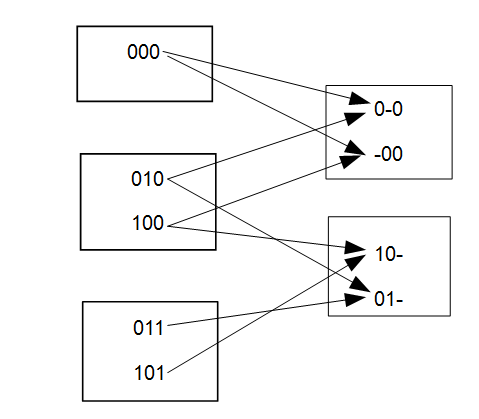
\includegraphics{images/51.png}
\end{center}

Второй шаг — это поиск минимального покрытия строками таблицы Квайна (импликантной таблицы). Наиболее мощным и универсальным является метод функций Петрика, но его недостатком является большой объѐм вычислений. В нашем случае таблица Квайна имеет вид:

\begin{center}
    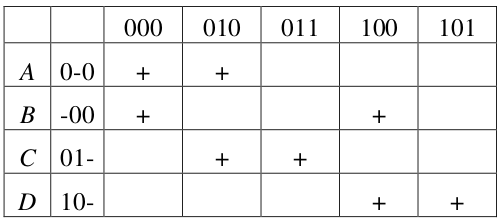
\includegraphics{images/52.png}
\end{center}

В первой строке таблицы стоят слагаемые СДНФ, а в первом столбце перечислены простые импликанты. Знаки «+» стоят там, где простая импликанта содержит данное слагаемое СДНФ. Составим и приведѐм к дизъюнктивной форме в соответствии с правилами раскрытия скобок и поглощения функцию Петрика. Для составления функции Петрика надо для каждого столбца взять дизъюнкцию простых импликант, отмеченных «+», и перемножить получившиеся выражения:

$K = (A \lor B)(A \lor C)C(B \lor D)D = (A \lor B)((A \lor C)C)((B \lor D)D) = (A \lor B)CD = ACD \lor BCD$

Каждому слагаемому теперь соответствует тупиковая ДНФ, конъюнкции надо заменить на дизъюнкции. В нашем случае обе ТДНФ являются минимальными:

МДНФ1=$A \lor C \lor D = \overline{x} \overline{z} \lor \overline{x} y \overline{x} y;$ МДНФ2=$B \lor C \lor D = \overline{y} \overline{z} \lor \overline{x} y \lor x \overline{y}$

Запишем результат в скобочной форме: $\overline{x} \overline{z} \lor \overline{x} y \lor x \overline{y} = \overline{x} (\overline{z} \lor y) \lor x \overline{y}$, $\overline{yz} \lor \overline{x} y \lor x \overline{y} = \overline{y} (\overline{z} \lor x) \lor \overline{x} y$


\end{document}